\subsection{Motorer og sensorer}
Ved testen som set på figur \ref{fig:HW_bipolar_akse} formåede den bipolære motor at drive aksen med små ophold.
\\
\\
Tabel \ref{tab:motor_moment} viser forskellen i moment for henholdsvis uni- og bipolær motor. Den bipolære motors moment er 118\% mere end den unipolæres. Resultaterne er udregnet ud fra testen med stativet fra figur \ref{fig:HW_stativ_test}. Se dokumentationen for test af bipolære motorer i bilagene.

\begin{table}[H]
  	\centering
	\begin{tabular}{ |l|c|c| }
  		\hline
  		\textbf{28BYJ-48} & Unipolær & Bipolær\\
  		\hline
  		Moment i full-step mode & 363 gcm & 792 gcm \\
  		\hline
	\end{tabular}
	\caption[]{Moment for 28BYJ-48\footnotemark}
	\label{tab:motor_moment}
\end{table}
\footnotetext{Dokumentation for test af motorer} 

\noindent
Figur \ref{Sensor_10cm} viser detektering af et objekt ved 10 cm afstand. Værdien 2241 er i mV. Figur 4 i databladet for sensoren viser ca. 2300 mV ved samme afstand hvilket giver en afvigelse på 2,57\% eller en unøjagtighed på 2,57 mm.

\begin{figure}[H]
	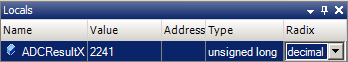
\includegraphics[scale=1]{tex/Test/Motor-sensor/Sensor_10cm.png}
	\caption{Resultat af detektering fra sensor ved 10 cm}
	\label{Sensor_10cm}
\end{figure}